\documentclass{beamer}
\usetheme{metropolis}
\usepackage[utf8]{inputenc}

\title{\VyZX}
\subtitle{Formal Verification of a Graphical Language}
\author{Adrian Lehmann \and \textbf{Benjamin Caldwell} \and Bhakti Shah \and Robert Rand}
\institute{Department of Computer Science \\ University of Chicago}
\date{}

\usepackage{underscore}           % Only needed if you use pdflatex.

\usepackage{amsthm}

\newtheorem{dfn}{Definition}

\usepackage{amsmath}
\usepackage{amssymb}
\usepackage{braket}
\usepackage{fancyhdr}
\usepackage{booktabs}

\usepackage[T1]{fontenc}
\usepackage[utf8]{inputenc}
\usepackage{regexpatch}
\usepackage{letltxmacro}
\usepackage{aligned-overset}

\usepackage{hyperref}
\usepackage[noabbrev,nameinlink]{cleveref}

\usepackage{enumitem}

\usepackage{xspace}

\usepackage{nowidow}
\usepackage{microtype}

\usepackage{float}
\usepackage{caption}
\usepackage{subcaption}

\usepackage{xcolor}
%\newcommand{\todo}[1]{{\color{red}\textbf{#1}}}{}


\usepackage{cancel}

\usepackage{algorithm}
\usepackage[noend]{algpseudocode}

\usepackage{wrapfig}

\usepackage{svg}

\usepackage{tikz}

\usepackage{stmaryrd}

\usetikzlibrary{backgrounds}
\usetikzlibrary{arrows}
\usetikzlibrary{shapes,shapes.geometric,shapes.misc}
\usetikzlibrary{decorations.pathmorphing}
\usetikzlibrary{decorations.pathreplacing}
\usetikzlibrary{decorations.markings}

\tikzstyle{every picture}=[baseline=-0.25em,scale=0.5]

\pgfkeys{/tikz/tikzit fill/.initial=0}
\pgfkeys{/tikz/tikzit draw/.initial=0}
\pgfkeys{/tikz/tikzit shape/.initial=0}
\pgfkeys{/tikz/tikzit category/.initial=0}

\newcommand{\tikzfig}[1]{%
\IfFileExists{#1.tikz}
  {\input{#1.tikz}}
  {%
    \IfFileExists{./figures/#1.tikz}
      {\input{./figures/#1.tikz}}
      {\tikz[baseline=-0.5em]{\node[draw=red,font=\color{red},fill=red!10!white] {\textit{#1}};}}%
  }%
}
\newcommand{\ctikzfig}[1]{%
\begin{center}\rm
  \tikzfig{#1}
\end{center}}

\newcommand{\hmaxtikzfig}[1]{\centering\resizebox{\textwidth}{!}{\tikzfig{#1}}}

\newcommand{\vmaxtikzfig}[1]{\centering\resizebox{!}{3.0cm}{\tikzfig{#1}}}

\newcommand{\pngfig}[2]{%
\IfFileExists{#1.png}
  {\includegraphics[width=#2]{./figures/#1.png}}
  {%
    \IfFileExists{./figures/#1.png}
      {\includegraphics[width=#2]{./figures/#1.png}}
      {\tikz[baseline=-0.5em]{\node[draw=red,font=\color{red},fill=red!10!white] {\textit{#1}};}}%
  }%
}

\newcommand{\cpngfig}[2]{
    \begin{center}
        \pngfig{#1}{#2}
    \end{center}
}

\newcommand{\oftype}[2]{\text{#1}\,:\,\text{#2}}
\newcommand{\ZX}[2]{\texttt{ZX}\,\,\text{#1}\,\,\text{#2}}
\newcommand{\nat}{\texttt{nat}}

\newcommand{\VyZX}{\textsl{Vy}\textsc{ZX}\xspace}
\newcommand{\SQIR}{\textsc{sqir}\xspace}
\newcommand{\QASM}{\texttt{QASM}\xspace}
\newcommand{\QLib}{\texttt{QuantumLib}\xspace}
\newcommand{\pyZX}{PyZX\xspace}
\newcommand{\VOQC}{\textsc{Voqc}\xspace}
\newcommand{\QWIRE}{\texttt{QWIRE}\xspace}
\newcommand{\inQWIRE}{\texttt{inQWIRE}\xspace}
\newcommand{\certiq}{\texttt{CertiQ}\xspace}
\newcommand{\tket}{\texttt{t\(\ket{\text{ket}}\)}\xspace}
\newcommand{\quartz}{Quartz\xspace}

% links formatting
\hypersetup{
    colorlinks,
    linkcolor={red!50!black},
    citecolor={blue!50!black},
    urlcolor={blue!80!black}
}



\usepackage{mathpartir}
% Comments
\usepackage{etoolbox}

\definecolor{zxred}{RGB}{0.9, 0.65, 0.65}
\definecolor{zxgreen}{RGB}{0.85, 0.97, 0.85}
\definecolor{egreen}{rgb}{0.31, 0.78, 0.47}
\definecolor{ate}{rgb}{0.58, 0.0, 0.83}
\newtoggle{revision}
%\toggletrue{revision}
\togglefalse{revision}

\iftoggle{revision}{
    \newcommand{\rnr}[1]{\textit{\textcolor{blue}{Robert: #1}}}
    \newcommand{\ael}[1]{\textit{\textcolor{purple}{Adrian: #1}}}
    \newcommand{\ben}[1]{\textit{\textcolor{egreen}{Ben: #1}}}
    \newcommand{\todo}[1]{\textit{\textcolor{red}{TODO: #1}}}
    %%%% Refcheck
    
    \usepackage{refcheck}
    
    %%% Infrastructure    
    \makeatletter
    \newcommand{\refcheckize}[1]{%
      \expandafter\let\csname @@\string#1\endcsname#1%
      \expandafter\DeclareRobustCommand\csname relax\string#1\endcsname[1]{%
        \csname @@\string#1\endcsname{##1}\wrtusdrf{##1}}%
      \expandafter\let\expandafter#1\csname relax\string#1\endcsname
    }
    \makeatother
    %%%
    
    %%% Now we add the reference commands we want refcheck to be aware of
    \refcheckize{\cref}
    \refcheckize{\Cref}
}{
    \newcommand{\rnr}[1]{}
    \newcommand{\ael}[1]{}
    \newcommand{\ben}[1]{}
    \newcommand{\todo}[1]{}
}


\newcommand{\R}{\mathbb{R}}
\newcommand{\C}{\mathbb{C}}
\newcommand{\N}{\mathbb{N}}

\pgfdeclarelayer{edgelayer}
\pgfdeclarelayer{nodelayer}
\pgfsetlayers{background, edgelayer, nodelayer, main}
\tikzstyle{none}=[inner sep=0mm]
\tikzstyle{every loop}=[]
\tikzstyle{mark coordinate}=[inner sep=0pt,outer sep=0pt,minimum size=3pt,fill=black,circle]
\input{zh.tikzdefs}
\input{zh.tikzstyles}


\algnewcommand\algorithmicswitch{\textbf{switch}}
\algnewcommand\algorithmiccase{\textbf{case}}
\algnewcommand\algorithmicassert{\texttt{assert}}

\algdef{SE}[SWITCH]{Switch}{EndSwitch}[1]{\algorithmicswitch\ #1\ \algorithmicdo}{\algorithmicend\ \algorithmicswitch}%
\algdef{SE}[CASE]{Case}{EndCase}[1]{\algorithmiccase\ #1}{\algorithmicend\ \algorithmiccase}%
\algtext*{EndSwitch}%
\algtext*{EndCase}%

\makeatletter
\def\blfootnote{\gdef\@thefnmark{}\@footnotetext}
\makeatother

\newcommand{\mailtodomain}[1]{\href{mailto:#1}{\nolinkurl{#1}}}


\metroset{block=fill}
\newcommand{\labelitemi}{$\circ$}

\begin{document}

\begin{frame}
  \maketitle
\end{frame}

\begin{frame}
  \frametitle{Why Verify?}

  Interactive proof is a useful tool to assist our reasoning process

  \pause

  Fully Axiomatic:
  \begin{itemize}
      \item Quantomatic (https://quantomatic.github.io/)
      \item ZX Calculator (zx.cduck.me)
      \item Chyp (https://github.com/akissinger/chyp)
  \end{itemize}

  \pause 

  We want instead to embed the ZX-Calculus in a proof assistant without axiomatizing anything.

\end{frame}

\begin{frame}
  \frametitle{Why Coq?}

  Three primary benefits
  \begin{itemize}
    \item Extraction
    \item SQIR
    \item QuantumLib
  \end{itemize}

  \break

  \begin{block}{Research Question}
    How can we embed a diagrammatic language (The ZX-Calculus) into Coq in a way that best utilizes the existing tools in Coq?
  \end{block}

\end{frame}

\begin{frame}
  \frametitle{Our Approach}

  Diagrams must have a ``semantic backing'', a function that evaluates diagrams as matrices

  Enables:
  \begin{itemize}
    \item Smaller core of truth
    \item Verified conversions between circuits and diagrams
    \item Easy to state equivalence of diagrams based on equivalence of semantics
  \end{itemize}

  \pause

  Downside:
  \begin{itemize}
    \item Difficult to apply semantics to a undirected and potentially cyclic graph
  \end{itemize}

\end{frame}

\begin{frame}
  \frametitle{Easy Form for Diagram Computation}

  A common trick to compute semantics for a diagram is to break them down into single pieces that are stacked together and composed horizontally.
  %
  You can also arrive here using the language of category theory.
  
  We take this inspiration to define a simple structure that we can define semantics for in Coq.

  \begin{figure}
    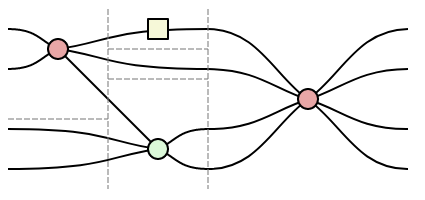
\includegraphics[width=50mm]{figures/smaller.png}
    \caption{An image from the \zxcalculus website tutorial with the caption ``An indication of how to break a diagram down into smaller diagrams, so that each cell contains only one element''}
  \end{figure}

\end{frame}

\begin{frame}{ZX Diagrams as string diagrams}
    \hmaxtikzfig{diagram-parts}
\end{frame}



\begin{frame}{Inductive ZX Diagrams}
    
    To define our ZX diagrams, we take these string diagram constructions and \alert{add Z and X spiders}.
    
    \begin{figure}[t]
    \centering
            
            \begin{subfigure}{.4\textwidth}
            \inferrule
            {\oftype{in out}{\(\N\)} \and \oftype{\(\alpha\)}{\(\R\)}}
            {\oftype{\texttt{Z_Spider} in out \(\alpha\)}{\ZX{in}{out}}}
            \end{subfigure}\hfill\begin{subfigure}{.4\textwidth}
            \inferrule
            {\oftype{in out}{\(\N\)} \and \oftype{\(\alpha\)}{\(\R\)}}
            {\oftype{\texttt{X_Spider} in out \(\alpha\)}{\ZX{in}{out}}}
            \end{subfigure}
            
            \begin{subfigure}{.25\textwidth}
            \inferrule{ }{\oftype{\texttt{Cap}}{\ZX{0}{2}}}
            \end{subfigure}\hfill\begin{subfigure}{.25\textwidth}
            \inferrule{ }{\oftype{\texttt{Cup}}{\ZX{2}{0}}}
            \end{subfigure}\hfill\begin{subfigure}{.25\textwidth}
            \inferrule{ }{\oftype{\texttt{Swap}}{\ZX{2}{2}}}
            \end{subfigure}\hfill\begin{subfigure}{.25\textwidth}
            \inferrule{ }{\oftype{\texttt{Empty}}{\ZX{0}{0}}}
            \end{subfigure}
            
            \begin{subfigure}{.6\textwidth}
            \inferrule
            {\oftype{zx1}{\ZX{in}{mid}} \and \oftype{zx2}{\ZX{mid}{out}}}
            {\oftype{\texttt{Compose} zx1 zx2}{\ZX{in}{out}}}
            \end{subfigure}\hfill\begin{subfigure}{.4\textwidth}
                \inferrule{ }{\oftype{\texttt{Wire}}{\ZX{1}{1}}}
            \end{subfigure}
            
            \begin{subfigure}{.6\textwidth}
            \inferrule
            {\oftype{zx1}{\ZX{in1}{out1}} \and \oftype{zx2}{\ZX{in2}{out2}}}
            {\oftype{\texttt{Stack} zx1 zx2}{\ZX{(in1 + in2)}{(out1 + out2)}}}
            \end{subfigure}\hfill\begin{subfigure}{.4\textwidth}
                \inferrule{ }{\oftype{\texttt{Box}}{\ZX{1}{1}}}
            \end{subfigure}

        \label{fig:blockconstructors}
    \end{figure}
\end{frame}

\begin{frame}{Semantics}

    To verify transformations on diagrams, we introduce a semantic function for our diagrams, $\llbracket \bullet \rrbracket ::$ \ZX{n}{m} $\to$ $\mathbb{C}^{m\times n}$. These semantics are built on the Coq library QuantumLib.
    
    \begin{align*}
        \llbracket\texttt{Z_Spider n m }\alpha\rrbracket \quad &\mapsto \hspace{47pt}
        \begin{bmatrix} 
            1 & \dotsi & 0 \\ 
            \vdots & \ddots & 0 \\ 
            0 & 0 & e^{i\alpha}
        \end{bmatrix}
    \\
    \llbracket\texttt{X_Spider n m }\alpha\rrbracket  \quad &\mapsto \quad H^{\otimes m} \times 
        \begin{bmatrix} 
            1 & \dotsi & 0 \\ 
            \vdots & \ddots & 0 \\ 
            0 & 0 & e^{i\alpha}
        \end{bmatrix} \times H^{\otimes n}
    \end{align*}
\end{frame}
    
\begin{frame}{More Semantics}
    \begin{align*}
        \llbracket\texttt{Cap}\rrbracket &\mapsto 
        \begin{bmatrix} 
            1 & 0 & 0 & 1
        \end{bmatrix}
    \\
        \llbracket\texttt{Cup}\rrbracket &\mapsto 
        \begin{bmatrix} 
            1 & 0 & 0 & 1
        \end{bmatrix}^\top
    \\
        \llbracket\texttt{Swap}\rrbracket &\mapsto
        \begin{bmatrix}
            1 & 0 & 0 & 0 \\
            0 & 0 & 1 & 0 \\
            0 & 1 & 0 & 0 \\
            0 & 0 & 0 & 1
        \end{bmatrix}
    \\
        \llbracket\texttt{Empty}\rrbracket &\mapsto
        \begin{bmatrix}
            1
        \end{bmatrix}
    \\   
        \llbracket\texttt{Wire}\rrbracket &\mapsto I_{2\times 2}
    \\
        \llbracket\texttt{Box}\rrbracket &\mapsto H
    \\
        \llbracket\texttt{Compose zx1 zx2}\rrbracket &\mapsto 
        \llbracket\texttt{zx2}\rrbracket \times \llbracket\texttt{semantics(zx1)}\rrbracket
    \\
        \llbracket\texttt{Stack zx1 zx2}\rrbracket &\mapsto
        \llbracket\texttt{semantics(zx1)}\rrbracket \otimes \llbracket\texttt{semantics(zx2)}\rrbracket
    \end{align*}
\end{frame}

\begin{frame}{Proportionality}

  We choose to define proportionality up to constant factor as follows, using the notation $\propto$.
  \[
      \exists c \neq 0: \llbracket zx1 \rrbracket = c * \llbracket zx2 \rrbracket \implies zx1 \propto zx2
  \]
  
  We can encode this proportionality definition in Coq easily using the inductive definition and semantic function defined earlier.

\end{frame}

\begin{frame}
  \frametitle{Utilizing Coq's Rewrite System}

  Proof in Coq has 3 important parts:
  \begin{itemize}
    \item Tactics
    \item Hypotheses
    \item Goal
  \end{itemize}

  The hypotheses and goal make up the proof state, while tactics are applied line by line to update the proof state.

\end{frame}

\begin{frame}
  \frametitle{Proof Example}

  Proofs in Coq must first be stated using keywords like \textit{Lemma} then proofs are surrounded by \textit{Proof} and \textit{Qed}.
  %
  Each line of a Coq proof has an associated proof state, and tactics operate and update these proof states.

  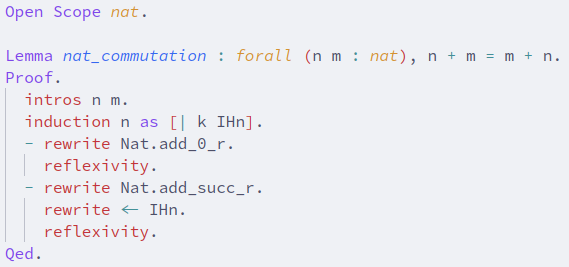
\includegraphics[width = \linewidth]{figures/coqproof.png}

\end{frame}

\begin{frame}
  \frametitle{Goal and Hypotheses Example}

  Goals and hypotheses are rendered based on the currently active line.

  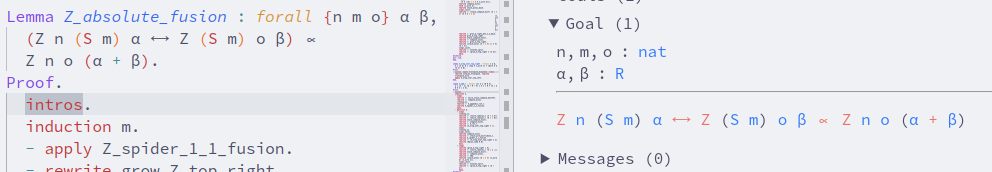
\includegraphics[width = \linewidth]{figures/goalhypotheses.png}

  This form ends up being difficult to read, so we have a VSCode extension which works with the language server to render diagrams.

\end{frame}

\begin{frame}
  \frametitle{Blocky Renderings}

  \texttt{Z n (S m) $\alpha$ $\leftrightarrow$ Z (S m) o $\beta$ $\propto$ Z n o $(\alpha + \beta)$}

  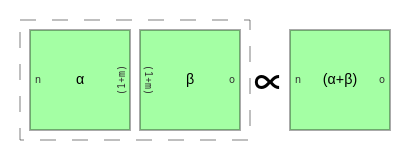
\includegraphics[width = \linewidth]{figures/fusionrender.png}

\end{frame}

\begin{frame}
  \frametitle{Associativity information}

  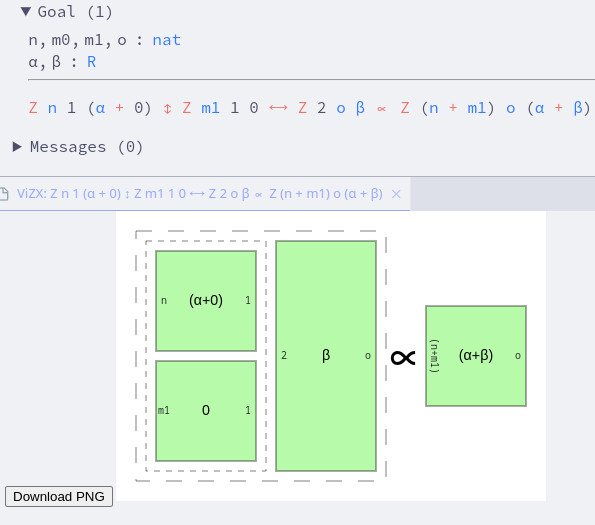
\includegraphics[width = \linewidth]{figures/stackcomposeex.png}

\end{frame}

\begin{frame}
  \frametitle{Tactics: Rewrite}

  Given a goal state $G$ and a hypothesis $Hyp : G = H$, we can apply the tactic \texttt{rewrite G} to update our proof state to be $H$.

  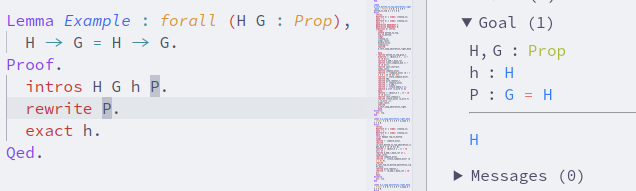
\includegraphics[width = \linewidth]{figures/rewriteex.png}

  We extend $\propto$ so that it can rewrite within ZX-diagrams using a tool within Coq called \textit{parametric relations} and \textit{parametric morphisms}.

\end{frame}

\begin{frame}
  \frametitle{Tactics: Apply}

  Given a goal state $G$ and a hypothesis $Hyp : H \to G$, we can use the tactic \texttt{apply Hyp} to update our proof state to be $H$.
  
  \begin{center}
    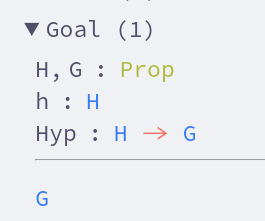
\includegraphics[width = 50mm]{figures/applyexample.png}
  \end{center}

\end{frame}

\begin{frame}{Three Proof Strategies}

    1. Proof through \alert{semantics}
    \ctikzfig{identity-base}

    \pause

    2. \alert{Inductive} proof
    \ctikzfig{absolutefusion} 

    \pause

    3. \alert{Diagrammatic} proof
    \ctikzfig{bell-pair-highlevel}

    
\end{frame}

\begin{frame}
  \frametitle{Current Features}

  \begin{itemize}
    \item Complete set of rewrite rules proven in Coq
    \item Automation to simplify diagrams
    \item Reasoning about 
  \end{itemize}

\end{frame}

\begin{frame}{Discussion}
    \begin{itemize}
        \item Any ZX diagram can be expressed
        \item Multiple ways to encode
        \item Deal with associativity information
        \item Dimensionality issues
        \item Complete set of rules have been verified, still there are reasonsa to do proof via semantics.
    \end{itemize}
\end{frame}

\begin{frame}{How can I verify my graphical language?}
    \begin{itemize}
        \item Find underlying categorical structure 
        \item Formally extend structure with generators
        \item Translate into inductive constructors
        \item Define a semantic for the inductive constructors
        \item Deal with resulting associtativity issues
    \end{itemize}

    \pause 

    We have separated the category theory work from VyZX into its own project, ViCaR. ViCaR also includes proofs that VyZX satisfies the definitions of dagger compact categories!

\end{frame}

\begin{frame}{Future work}
    \begin{itemize}
        \item Restore connection information, potentially have connection information generate these blocky diagrams.
        \item Verify ZX-based compiler.
        \item Rewriting diagrams without having to worry about associativity information.
    \end{itemize}
\end{frame}

\begin{frame}{Summary}
    \begin{itemize}
        \item Defined ZX diagrams inductively
        \item Inspired by string diagrams
        \item Multiple proof strategies
    \end{itemize}

    \begin{block}{Find \VyZX on GitHub}
        \centering \url{https://github.com/inQWIRE/VyZX}
    \end{block}

    \begin{block}{arXiv}
        \centering \url{https://arxiv.org/abs/2311.11571}
    \end{block}
    
\end{frame}




\begin{frame}{References}

    \bibliographystyle{amsalpha}
    \nocite{vandewetering2020zxcalculus}
    \nocite{coecke-kissinger-2017-picturing-q-proc}
    \nocite{castello2023inductive}
    \nocite{hietala-et-al-2021-VOQC}
    \bibliography{generic.bib}

\end{frame}

\end{document}
